\documentclass[11pt,a4paper]{article}  % Déclare la classe du document.

\newcommand{\chaptermark}[2]{\og #2 \fg{} (#1)} % ligne uniquement pour éviter une erreur en cas d'article
\usepackage[table,dvipsnames,svgnames]{xcolor}
\usepackage{listingsutf8}
%\usepackage[utf8]{inputenc}% gestion des accents (source)
\usepackage[T1]{fontenc}% gestion des accents (PDF)
\usepackage{fontspec}
\usepackage[french]{babel}% gestion du français
\usepackage{textcomp}% caractères additionnels
\usepackage{mathtools,amssymb,amsthm}% packages de l'AMS + mathtools
\usepackage{amsmath}
\usepackage{yhmath}
\usepackage{mathpazo}
\usepackage[scaled=0.95]{helvet}
\usepackage{courier}
%\usepackage{fourier}
%\usepackage[scaled=0.95]{helvet}
%\usepackage{courier}
\usepackage{bm}
\usepackage{gensymb}
\usepackage{graphicx}

\usepackage{enumitem}
\usepackage{pifont}

\usepackage{pstricks}
\usepackage{pstricks-add}
\usepackage{pst-eucl}
\usepackage{pgfplots}
\let\clipbox\relax
%\usepackage{pst-plot,pst-text,pst-tree,pstricks-add}
%\usepackage{pst-node} % required package
\usepackage{pst-all}
\usepackage[most,skins,breakable]{tcolorbox}

\usepackage{euscript}





% ############### Nouvelles commandes ###############
% Coloration des labels des points dans pst-eucl
\makeatletter
\define@key[psset]{pst-eucl}{LabelColor}{\def\psk@LabelColor{#1}}
\psset{LabelColor=black}
\def\Pst@WhichLabel#1{{\color{\psk@LabelColor}%
		\ifx\psk@PointName\@default#1\else\psk@PointName\fi}}
\makeatother

% renomme le symbole #2 en #1#2 et invalide le symbole initial #2:
\def\renamesymbol#1#2{
	\expandafter\let\expandafter\newsym\expandafter=\csname#2\endcsname
	\expandafter\global\expandafter\let\csname#1#2\endcsname=\newsym
	\expandafter\global\expandafter\let\csname#2\endcsname=\origsym
}



\usepackage{ProfCollege}
\renamesymbol{Casio}{Calculatrice}
\usepackage[nonshellescape]{ProfLycee}



%\usepackage[left=1.5cm,right=1.5cm,top=2.5cm,bottom=2.5cm]{geometry}
\usepackage[left=13mm,right=13mm,top=18mm,bottom=18mm,footskip=30pt]{geometry}
\setlength{\headheight}{15pt}

\usepackage{titlesec}
\usepackage{pas-math}
\usepackage{longtable}
\usepackage{tikz,tkz-tab}
\usepackage{amsmath}
\usepackage[right]{eurosym}
\usepackage{sectsty}
\usepackage{tipfr}
\usepackage{setspace}

%pour faire les touches de la calculatrices
\usepackage{menukeys}
\renewmenumacro{\menu}{roundedmenus} % default: menus
\renewmenumacro{\directory}{pathswithfolder} % default: paths
\renewmenumacro{\keys}{shadowedroundedkeys} % default: roundedkeys


\usepackage{multicol}
\usepackage{multirow}
\usepackage{systeme}

%% Format des titres de chapitres, paragraphes, ...
\titleformat{\chapter}[frame]
{\color{red!85!white}\normalsize}%
{\filright\sffamily\Large%
	\enspace Chapitre \thechapter\enspace}%
{8pt}
{\color{red!85!white}\rule{0pt}{30pt}\sffamily\Huge\bfseries\filcenter}
%%%%%%%%%%%%%%%%%%%%
\titlespacing{\chapter}{0pc}{0pc}{2pc}
\titlespacing{\subsection}{2pc}{}{}

\titleformat{\subsection}[block]{\hspace{1em}}{\thesubsection}{1em .}{}
\titleformat{\subsubsection}[block]{\hspace{2em}}{\thesubsection}{1em )}{}

\chapterfont{\color{red}{}}
\sectionfont{\color{green!55!black}{}}
\subsectionfont{\color{cyan!65!black}{}}
\subsubsectionfont{\color{violet}{}}
\renewcommand{\thesection}{\color{green!55!black}\Roman{section}.}
\renewcommand{\thesubsection}{\color{cyan!65!black}\arabic{subsection})}
\renewcommand{\thesubsubsection}{\color{violet}\alph{subsubsection})}
\setcounter{secnumdepth}{3}

\titleformat{\subsection}[block]{\hspace{1em}}{\thesubsection}{1em .}{}
\titleformat{\subsubsection}[block]{\hspace{2em}}{\thesubsection}{1em )}{}

\usepackage[column=A]{cellspace}
\setlength{\cellspacebottomlimit}{4pt}
\setlength{\cellspacetoplimit}{4pt}
\setlength{\parindent}{2pt}
\setlength{\tabcolsep}{0.5cm}


%entête et pieds de pages
\usepackage{fancyhdr}
\pagestyle{fancy}
\fancyhf{}
\usepackage{lastpage}
\renewcommand{\chaptermark}[1]{\markboth {Chapitre \thechapter~ - ~#1}{}}
\renewcommand\headrulewidth{1pt}
\fancyhead[LO,RE]{Terminale $-$ Maths complémentaire}
\fancyhead[RO,LE]{\leftmark}
\renewcommand\footrulewidth{1pt}
\fancyfoot[LO,RE]{Année 2026-2027}
\fancyfoot[RO,LE]{\textbf{Page \thepage/\pageref{LastPage}}}

%Mes boites pour les définitions, propriétés, remarques, ...

%Mes boites pour les définitions, propriétés, remarques, ...

\newcommand\titrebox[1]{\textbf{#1}}
\newtcolorbox{definition}{breakable,colback=red!10!white,
	colframe=red!85!white, fonttitle=\bfseries,enhanced,
	attach boxed title to top left={xshift=5mm, yshift=-2mm},boxed title style={size=small,colback=red!10!white,colframe=red!85!white, arc=0.5mm},
	title=\textcolor{red!85!white}{Définition} , arc=3mm}

\newtcolorbox{definitionTitre}[1]{breakable,colback=red!10!white,
	colframe=red!85!white, fonttitle=\bfseries,enhanced,
	attach boxed title to top left={xshift=5mm, yshift=-2mm},boxed title style={size=small,colback=red!10!white,colframe=red!85!white, arc=0.5mm},
	title=\textcolor{red!85!white}{Définition - #1} , arc=3mm}

\newtcolorbox{definitionPerso}[1]{breakable,colback=red!10!white,
	colframe=red!85!white, fonttitle=\bfseries,enhanced,
	attach boxed title to top left={xshift=5mm, yshift=-2mm},boxed title style={size=small,colback=red!10!white,colframe=red!85!white, arc=0.5mm},
	title=\textcolor{red!85!white}{#1} , arc=3mm}

\newtcolorbox{regle}{breakable,colback=red!10!white,
	colframe=red!85!white, fonttitle=\bfseries,enhanced,
	attach boxed title to top left={xshift=5mm, yshift=-2mm},boxed title style={size=small,colback=red!10!white,colframe=red!85!white, arc=0.5mm},
	title=\textcolor{red!85!white}{Règle} , arc=3mm}

\newtcolorbox{regles}{breakable,colback=red!10!white,
	colframe=red!85!white, fonttitle=\bfseries,enhanced,
	attach boxed title to top left={xshift=5mm, yshift=-2mm},boxed title style={size=small,colback=red!10!white,colframe=red!85!white, arc=0.5mm},
	title=\textcolor{red!85!white}{Règles} , arc=3mm}

\newtcolorbox{definitions}{breakable,colback=red!10!white,
	colframe=red!85!white, fonttitle=\bfseries,enhanced,
	attach boxed title to top left={xshift=5mm, yshift=-2mm},boxed title style={size=small,colback=red!10!white,colframe=red!85!white, arc=0.5mm},
	title=\textcolor{red!85!white}{Définitions} , arc=3mm}

\newtcolorbox{propriete}{breakable,colback=red!10!white,
	colframe=red!85!white, fonttitle=\bfseries,enhanced,
	attach boxed title to top left={xshift=5mm, yshift=-2mm},boxed title style={size=small,colback=red!10!white,colframe=red!85!white, arc=0.5mm},
	title=\textcolor{red!85!white}{Propriété} , arc=3mm}

\newtcolorbox{proprieteTitre}[1]{breakable,colback=red!10!white,
	colframe=red!85!white, fonttitle=\bfseries,enhanced,
	attach boxed title to top left={xshift=5mm, yshift=-2mm},boxed title style={size=small,colback=red!10!white,colframe=red!85!white, arc=0.5mm},
	title=\textcolor{red!85!white}{Propriété - #1} , arc=3mm}

\newtcolorbox{proprietes}{breakable,colback=red!10!white,
	colframe=red!85!white, fonttitle=\bfseries,enhanced,
	attach boxed title to top left={xshift=5mm, yshift=-2mm},boxed title style={size=small,colback=red!10!white,colframe=red!85!white, arc=0.5mm},
	title=\textcolor{red!85!white}{Propriétés} , arc=3mm}

\newtcolorbox{theoreme}{breakable,colback=red!10!white,
	colframe=red!85!white, fonttitle=\bfseries,enhanced,
	attach boxed title to top left={xshift=5mm, yshift=-2mm},boxed title style={size=small,colback=red!10!white,colframe=red!85!white, arc=0.5mm},
	title=\textcolor{red!85!white}{Théorème} , arc=3mm}

\newtcolorbox{theoremeTitre}[1]{breakable,colback=red!10!white,
	colframe=red!85!white, fonttitle=\bfseries,enhanced,
	attach boxed title to top left={xshift=5mm, yshift=-2mm},boxed title style={size=small,colback=red!10!white,colframe=red!85!white, arc=0.5mm},
	title=\textcolor{red!85!white}{Théorème - #1} , arc=3mm}

\newtcolorbox{theoremes}{breakable,colback=red!10!white,
	colframe=red!85!white, fonttitle=\bfseries,enhanced,
	attach boxed title to top left={xshift=5mm, yshift=-2mm},boxed title style={size=small,colback=red!10!white,colframe=red!85!white, arc=0.5mm},
	title=\textcolor{red!85!white}{Théorèmes} , arc=3mm}

\newtcolorbox{bexemple}{
	enhanced,
	breakable,
	fonttitle=\bfseries,
	frame empty,
	nobeforeafter,
	borderline west={0.5mm}{0mm}{cyan!75!black},
	title=\textcolor{cyan!75!black}{\faHubspot\:\:Exemple},
	%title after break=Exemple (suite),
	colback=white,
	extras={enhanced, frame empty},
	detach title,before upper={\tcbtitle\ :\quad },
}

\newtcolorbox{bexemples}{
	enhanced,
	breakable,
	fonttitle=\bfseries,
	frame empty,
	nobeforeafter,
	borderline west={0.5mm}{0mm}{cyan!75!black},
	title=\textcolor{cyan!75!black}{\faHubspot\:\:Exemples},
	%title after break=Exemples (suite),
	colback=white,
	extras={enhanced, frame empty},
	detach title,before upper={\tcbtitle\ :\quad },
}

\newtcolorbox{bexemplet}[1]{
	enhanced,
	breakable,
	fonttitle=\bfseries,
	frame empty,
	borderline west={0.5mm}{0mm}{cyan!75!black},
	title=\textcolor{cyan!75!black}{\faHubspot\:\:Exemple - #1},
	colback=white,
	extras={enhanced, frame empty},
	detach title,before upper={\tcbtitle\ :\quad },
}

\newtcolorbox{brmq}{
	enhanced,
	breakable,
	fonttitle=\bfseries,
	frame empty,
	nobeforeafter,
	borderline west={0.5mm}{0mm}{orange!95!white},
	title=\textcolor{orange!85!white}{\faHandPointRight[regular]\:\:Remarque} ,
	colback=white,
	extras={enhanced, frame empty},
	detach title,before upper={\tcbtitle\ \quad },
}

\newtcolorbox{brmqs}{
	enhanced,
	breakable,
	fonttitle=\bfseries,
	frame empty,
	nobeforeafter,
	borderline west={0.5mm}{0mm}{orange!85!white},
	title=\textcolor{orange!85!white}{\faHandPointRight[regular]\:\:Remarques},
	colback=white,
	detach title,before upper={\tcbtitle\ \quad },
	extras={enhanced, frame empty},
}

\newtcolorbox{brmqt}[1]{
	enhanced,
	breakable,
	fonttitle=\bfseries,
	frame empty,
	nobeforeafter,
	borderline west={0.5mm}{0mm}{orange!85!white},
	title=\textcolor{orange!85!white}{\faHandPointRight[regular]\:\:Remarque - #1},
	colback=white,
	extras={enhanced, frame empty},
	detach title,before upper={\tcbtitle\ \quad },
}

\newtcolorbox{consequences}[1]{
	enhanced,
	breakable,
	fonttitle=\bfseries,
	frame empty,
	nobeforeafter,
	borderline west={0.5mm}{0mm}{ProcessBlue},
	title=\textcolor{ProcessBlue}{#1},
	colback=white,
	extras={enhanced, frame empty},
	detach title,before upper={\tcbtitle\ :\quad },
}

\newtcolorbox{bmethode}{
	enhanced,
	breakable,
	fonttitle=\bfseries,
	frame empty,
	nobeforeafter,
	borderline west={0.5mm}{0mm}{blue!75!black},
	title=\textcolor{blue!75!black}{Méthode} ,
	colback=white,
	extras={enhanced, frame empty},
	attach boxed title to top left = {xshift = -3mm},
	boxed title style={size=small,colback=white,colframe=blue!75!black, arc=3mm,
	}
}

\newtcolorbox{bmethodes}{
	enhanced,
	breakable,
	fonttitle=\bfseries,
	frame empty,
	nobeforeafter,
	borderline west={0.5mm}{0mm}{blue!75!black},
	title=\textcolor{blue!75!black}{Méthodes} ,
	colback=white,
	extras={enhanced, frame empty},
	attach boxed title to top left = {xshift = -3mm},
	boxed title style={size=small,colback=blue!75!black,colframe=blue!75!black, arc=3mm,
	}
	boxed title after break style={size=small,colback=white,colframe=blue!75!black, arc=3mm,
	}
}

\newtcolorbox{bmethodet}[1]{
	enhanced,
	breakable,
	fonttitle=\bfseries,
	frame empty,
	nobeforeafter,
	borderline west={0.5mm}{0mm}{blue!75!black},
	title=\textcolor{blue!75!black}{\faTasks\:\:Méthode - #1} ,
	colback=white,
	extras={enhanced, frame empty},
	attach boxed title to top left = {xshift = -3mm},
	boxed title style={size=small,colback=white,colframe=blue!75!black, arc=3mm,
	}
}

\newtcolorbox{bdemo}{
	enhanced,
	breakable,
	fonttitle=\bfseries,
	frame empty,
	nobeforeafter,
	borderline west={0.5mm}{0mm}{violet!65!white},
	title={\faEdit[regular]\:\:Démonstration},
	%title after break=Démonstration (suite),
	colback=white,
	extras={enhanced, frame empty},
	attach boxed title to top left = {xshift = -3mm},
	boxed title style={size=small,colback=violet!65!white,colframe=violet!65!white, arc=3mm,
	}
}

\newtcolorbox{bdemos}{
	enhanced,
	breakable,
	fonttitle=\bfseries,
	frame empty,
	nobeforeafter,
	borderline west={0.5mm}{0mm}{violet!65!white},
	title={\faEdit[regular]\:\:Démonstrations},
	%title after break=Démonstration (suite),
	colback=white,
	extras={enhanced, frame empty},
	attach boxed title to top left = {xshift = -3mm},
	boxed title style={size=small,colback=violet!65!white,colframe=violet!65!white, arc=3mm,
	}
}

\newtcolorbox{bdemot}[1]{
	enhanced,
	breakable,
	fonttitle=\bfseries,
	frame empty,
	nobeforeafter,
	borderline west={0.5mm}{0mm}{violet!65!white},
	title={\faEdit[regular]\:\:Démonstration - #1},
	%title after break=Démonstration (suite),
	colback=white,
	extras={enhanced, frame empty},
	attach boxed title to top left = {xshift = -3mm},
	boxed title style={size=small,colback=violet!65!white,colframe=violet!65!white, arc=3mm,
	}
}

\newtcolorbox{boxPerso}[2]{
	enhanced,
	breakable,
	fonttitle=\bfseries,
	frame empty,
	nobeforeafter,
	borderline west={0.5mm}{0mm}{#2},
	title=#1,
	%title after break=Exemple (suite),
	colback=white,
	extras={enhanced, frame empty},
	detach title,before upper={\tcbtitle\ :\quad },
}


\newcommand*{\Coord}[3]{% 
	\ensuremath{\vv{#1}\, 
		\begin{pmatrix} 
			#2\\ 
			#3 
\end{pmatrix}}}

\newcommand*{\CoordSV}[2]{% 
	\ensuremath{\begin{pmatrix} 
			#1\\ 
			#2 
\end{pmatrix}}}

\newcommand*{\Coordp}[3]{% 
	\ensuremath{\vv{#1}\, 
		\left\lvert 
		\begin{matrix} 
			#2\\ 
			#3 
		\end{matrix}  
		\right.% Ne pas oublier le délimiteur invisible. 
}}


%personnalisation des listes non numérotées pour les différentes boites 
\newlist{itemEx}{itemize}{2}
\setlist[itemEx,1]{label=$\bullet$, font=\color{cyan!75!black}}
\setlist[itemEx,2]{label=$\bullet$, font=\color{cyan!75!black}}

\newlist{enumEx}{enumerate}{2}
\setlist[enumEx,1]{label=\arabic*), font=\bf\color{cyan!75!black}}
\setlist[enumEx,2]{label=\alph*), font=\bf\color{cyan!75!black}}

\newlist{itemMet}{itemize}{2}
\setlist[itemMet,1]{label=$\bullet$, font=\color{blue!75!black}}
\setlist[itemMet,2]{label=$\bullet$, font=\color{blue!75!black}}

\newlist{enumMet}{enumerate}{2}
\setlist[enumMet,1]{label=\arabic*), font=\bf\color{blue!75!black}}
\setlist[enumMet,2]{label=\alph*), font=\bf\color{blue!75!black}}

\newlist{itemDef}{itemize}{2}
\setlist[itemDef,1]{label=$\bullet$, font=\color{ForestGreen}}
\setlist[itemDef,2]{label=$\bullet$, font=\color{ForestGreen}}

\newlist{enumDef}{enumerate}{2}
\setlist[enumDef,1]{label=\arabic*), font=\bf\color{ForestGreen}}
\setlist[enumDef,2]{label=\alph*), font=\bf\color{ForestGreen}}

\newlist{itemProp}{itemize}{2}
\setlist[itemProp,1]{label=$\bullet$, font=\color{red!85!white}}
\setlist[itemProp,2]{label=$\bullet$, font=\color{red!85!white}}

\newlist{enumProp}{enumerate}{2}
\setlist[enumProp,1]{label=\arabic*), font=\bf\color{red!85!white}}
\setlist[enumProp,2]{label=\alph*), font=\bf\color{red!85!white}}

\newlist{itemDem}{itemize}{2}
\setlist[itemDem,1]{label=$\bullet$, font=\color{violet!85!white}}
\setlist[itemDem,2]{label=$\bullet$, font=\color{violet!85!white}}

\newlist{enumDem}{enumerate}{2}
\setlist[enumDem,1]{label=\arabic*), font=\bf\color{violet!85!white}}
\setlist[enumDem,2]{label=\alph*), font=\bf\color{violet!85!white}}

\newlist{itemRem}{itemize}{2}
\setlist[itemRem,1]{label=\ding{43}, font=\color{orange!85!white}}
\setlist[itemRem,2]{label=\ding{43}, font=\color{orange!85!white}}

\newlist{enumRem}{enumerate}{2}
\setlist[enumRem,1]{label=\arabic*), font=\bf\color{orange!85!white}}
\setlist[enumRem,2]{label=\alph*), font=\bf\color{orange!85!white}}

% nouvelle commande pour mettre entre guillemets une expression
\newcommand{\guillemets}[1]{\og \emph{#1} \fg}


\newcommand{\corr}[1]{\fcolorbox{red}{yellow!30}{#1}}

\newtcolorbox{corrBox}{enhanced,breakable,boxrule=1pt,nobeforeafter,boxsep=0pt,left=\fboxsep,right=\fboxsep,colback=yellow!30,colframe=red!75!black}

% commandes pour mettre en couleur (et en gras) dans une expression mathématique.
\newcommand{\mVert}[1]{{\color{green!55!black}\bm{#1}}}
\newcommand{\mVertWB}[1]{{\color{green!55!black}#1}}
\newcommand{\mRouge}[1]{{\color{red!85!white}\bm{#1}}}
\newcommand{\mRougeWB}[1]{{\color{red!85!white}#1}}
\newcommand{\mBleu}[1]{{\color{blue!75!black}\bm{#1}}}
\newcommand{\mBleuWB}[1]{{\color{blue!75!black}#1}}
\newcommand{\mOrange}[1]{{\color{orange!75!white}\bm{#1}}}
\newcommand{\mOrangeWB}[1]{{\color{orange!75!white}#1}}
\newcommand{\mViolet}[1]{{\color{violet!85!white}\bm{#1}}}
\newcommand{\mVioletWB}[1]{{\color{violet!85!white}#1}}

%commandes pour les flèches de distributivité.
\newcommand{\tikzmarkBB}[2][]{ \tikz[remember picture, overlay, baseline=-0.5ex]\node[#1, left](#2){}; }
\newcommand{\flechePropV}[4][]{ \tikz[remember picture, overlay]\draw (#2)edge[bend left=90,min distance=1em, -stealth]node[midway, #1]{#4}(#3); }
\newcommand{\flechePropH}[4][]{ \tikz[remember picture, overlay]\draw (#2)edge[bend left=90, min distance=1em, -stealth]node[midway, #1]{#4}(#3); }
\newcommand{\flechePropHbas}[4][]{ \tikz[remember picture, overlay]\draw (#2)edge[bend left=-90, min distance=1em, -stealth]node[midway, #1]{#4}(#3); }


\lstdefinestyle{algo}{%
	inputencoding=utf8,
	mathescape,
	basicstyle=\footnotesize\ttfamily,
	numberstyle=\scriptsize\ttfamily\color{gray},
	showstringspaces=false,
	tabsize=2,
	numbers=left,
	framexleftmargin=8mm,
	xleftmargin=8mm,
	keepspaces=true,
	frame=lines,
	framerule=1pt,
	rulecolor=\color{green!50!black},
	backgroundcolor=\color{green!5},
	keywords = {Pour, allant, Si, alors, Sinon, Fin},    
	morecomment=[l][commentstyle]{//},
	commentstyle=\color{gray},
	classoffset=0,
	keywordstyle=\color{blue!75},
	classoffset=1,
	morekeywords = {Afficher},
	keywordstyle=\color{green!50!black},
	classoffset=0,
	morestring=[b]",
	stringstyle=\color{red!75},
	literate=
	{é}{{\'e}}{1}%
	{è}{{\`e}}{1}%
	{à}{{\`a}}{1}%
	{â}{{\^a}}{1}%%%
	{ç}{{\c{c}}}{1}%
	{œ}{{\oe}}{1}%
	{ù}{{\`u}}{1}%
	{É}{{\'E}}{1}%
	{È}{{\`E}}{1}%
	{À}{{\`A}}{1}%
	{Ç}{{\c{C}}}{1}%
	{Œ}{{\OE}}{1}%
	{Ê}{{\^E}}{1}%
	{ê}{{\^e}}{1}%
	{î}{{\^i}}{1}%
	{ï}{{\"i}}{1}%%%
	{ô}{{\^o}}{1}%
	{û}{{\^u}}{1}%
	{=}{$\leftarrow$}{1}%
	{==}{$={}$}{1}}


%  --------   Macro pour les exercices et leur numérotation  

\newcounter{exo}

\setcounter{exo}{1}

\newcommand{\exercice}[1]{\vskip 0.2cm\noindent{\bf \ Exercice \theexo {  #1 }}\addtocounter{exo}{1}}

\newcounter{rit}

\setcounter{rit}{1}

\newcommand{\rituel}[1]{\vskip 0.2cm\noindent{ \bf \ \underline{Rit. \therit {  #1 }}}\addtocounter{rit}{1}}

\newcommand{\raisedrule}[2][0em]{\leaders\hbox{\rule[#1]{1pt}{#2}}\hfill}

\newcounter{numexo}

\setcounter{numexo}{1}

\newcommand{\exerciceDS}[1]{\vskip 0.6cm\noindent\rule[+2pt]{1cm}{0.5pt}\ {\large\bf \ Exercice \thenumexo {  #1 }}\raisedrule[+2pt]{0.5pt}\null\addtocounter{numexo}{1}\par\vskip 0,4cm}

\newcommand{\bareme}[1]{\tikz\node[circle,draw,inner sep=1pt,outer sep=1pt, color=red]{\textbf{#1}};}

%  --------   Pour le langage Python

% Default fixed font does not support bold face
\DeclareFixedFont{\ttb}{T1}{txtt}{bx}{n}{12} % for bold
\DeclareFixedFont{\ttm}{T1}{txtt}{m}{n}{12}  % for normal

% Custom colors
\usepackage{color}
\definecolor{deepblue}{rgb}{0,0,0.5}
\definecolor{deepred}{rgb}{0.6,0,0}
\definecolor{deepgreen}{rgb}{0,0.5,0}

\usepackage{listings}

% Python style for highlighting
\newcommand\pythonstyle{\lstset{
		language=Python,
		basicstyle=\ttm,
		otherkeywords={self},             % Add keywords here
		keywordstyle=\ttb\color{deepblue},
		emph={MyClass,__init__},          % Custom highlighting
		emphstyle=\ttb\color{deepred},    % Custom highlighting style
		stringstyle=\color{deepgreen},
		frame=tb,                         % Any extra options here
		showstringspaces=false            % 
}}


% Python environment
\lstnewenvironment{python}[1][]
{
	\pythonstyle
	\lstset{#1}
}
{}

% Python for external files
\newcommand\pythonexternal[2][]{{
		\pythonstyle
		\lstinputlisting[#1]{#2}}}

% Python for inline
\newcommand\pythoninline[1]{{\pythonstyle\lstinline!#1!}}


% \begin{document}
	
	% \section{``In-text'' listing highlighting}
	
	% \begin{python}
		% class MyClass(Yourclass):
		%     def __init__(self, my, yours):
		%         bla = '5 1 2 3 4'
		%         print bla
		% \end{python}
	
	% \section{External listing highlighting}
	
	% \pythonexternal{demo.py}
	
	% \section{Inline highlighting}
	
	% Definition \pythoninline{class MyClass} means \dots
	
	% \end{document}

\definecolor{codegreen}{rgb}{0,0.6,0}
\definecolor{codegray}{rgb}{0.5,0.5,0.5}
\definecolor{codepurple}{rgb}{0.58,0,0.82}
\definecolor{backcolour}{rgb}{0.95,0.95,0.92}

\lstdefinestyle{myStyle}{
	backgroundcolor=\color{backcolour},   
	commentstyle=\color{codegreen},
	keywordstyle=\color{magenta},
	numberstyle=\tiny\color{codegray},
	stringstyle=\color{codepurple},
	basicstyle=\ttfamily\footnotesize,
	breakatwhitespace=false,         
	breaklines=true,                 
	captionpos=b,                    
	keepspaces=true,                 
	numbers=left,                    
	numbersep=5pt,                  
	showspaces=false,                
	showstringspaces=false,
	showtabs=false,                  
	tabsize=2
}

\lstset{style=myStyle}

\newcommand{\normeB}[1]{\left\Vert \vv{#1}\right\Vert}

\newcommand\grasmaths[1]{\symbf{#1}}
\newcommand\sfbmath[1]{\symbf{\symsfup{#1}}}
\definecolor{marron}{rgb}{0.64,0.16,0.16}
\definecolor{titrebleu}{rgb}{0,0,0.6}

\usepackage{tabularx}
\usepackage{wasysym}
% ===========================tableaux de base
\newcolumntype{R}[1]{>{\raggedleft\arraybackslash }b{#1}} 
\newcolumntype{L}[1]{>{\raggedright\arraybackslash }b{#1}}
\newcolumntype{C}[1]{>{\centering\arraybackslash }b{#1}}
\newcolumntype{M}[1]{>{\centering\arraybackslash }m{#1}} %doublecentrée
\renewcommand{\tabularxcolumn}[1]{m{#1}}
\newcolumntype{Y}{>{\centering\arraybackslash }X}

%=============================boîtes de cours
\usepackage{fontawesome5}
\newcommand\fontbox{\sffamily}
%\newcommand\titrebox[1]{\textbf{#1}}
\tcbuselibrary{breakable}
\tcbset{bdefaut/.style={%
		fonttitle=\fontbox,%
		enhanced,breakable,center,boxrule=1.25pt,drop shadow=black!33!white,%
		sharp corners=uphill,arc=12pt,before skip=12pt,after skip=12pt,%
		left=5pt,leftupper=5pt,top=1mm,bottom=1mm,%
		before upper=\leavevmode
	}
}
\NewDocumentCommand\bbnewbox{ m m m m O{#4} !O{} }{%nom + titre + icone + bordure/titre/fondtitre + couleur fond + options
	\DeclareTColorBox{#1}{ O{} }{%
		bdefaut,%
		colframe=#4,coltitle=#4!25!Black,colbacktitle=#4!35,colback=#5!10,%
		title={#3\:\:\titrebox{#2##1}},%
		#6
	}%
}

\bbnewbox{bdefi}{Définition}{\faIcon[regular]{comment-dots}}{ForestGreen}
\bbnewbox{bcor}{Corollaire}{\faIcon[regular]{comment-dots}}{ForestGreen}
\bbnewbox{bdefis}{Définitions}{\faIcon[regular]{comment-dots}}{ForestGreen}
\bbnewbox{bhumour}{Humour}{\faIcon[regular]{laugh-wink}}{Yellow}
%\bbnewbox{bprop}{Propriété}{\faCog}{Salmon}
\bbnewbox{bprop}{Propriété}{\faCog}{red!85!white}
\bbnewbox{bprops}{Propriétés}{\faCog}{red!85!white}
\bbnewbox{bcscq}{Conséquence}{\faArrowAltCircleRight[regular]}{Salmon}
\bbnewbox{bthm}{Théorème}{\faBullhorn}{FireBrick}
\bbnewbox{blog}{Logiciel}{\faDev}{CornflowerBlue}[white]
\bbnewbox{bhistoire}{Point histoire}{\faUniversity}{Chocolate}[white]

%\bbnewbox{brmq}{Remarque}{\faHandPointRight[regular]}{MidnightBlue}[white]
\bbnewbox{bexercice}{Exercice}{\faHubspot}{MidnightBlue}
%\bbnewbox{bexemple}{Exemple}{\faHubspot}{MediumTurquoise}
\bbnewbox{bvoc}{Vocabulaire}{\faList*[regular]}{YellowGreen}
\bbnewbox{bnota}{Notation}{\faList*}{YellowGreen}
\bbnewbox{bregle}{Règle}{\faList*}{YellowGreen}
\bbnewbox{bcadre}{Cadre}{\faInfoCircle}{Peru}
\bbnewbox{bidee}{Idée}{\faInfo}{LightBlue}
\bbnewbox{bintro}{Intro}{\faMarker}{LightSalmon}
\bbnewbox{billustr}{Illustration}{\faChartLine}{Crimson}[White]
\bbnewbox{bvideo}{}{\faIcon[regular]{file-video}}{teal}[White]
\bbnewbox{bbilan}{Bilan}{\faForward}{Purple}
%\bbnewbox{bmethode}{Méthode}{\faTasks}{Coral}
%\bbnewbox{bmethode}{Méthode}{\faTasks}{blue!75!black}
\bbnewbox{btuto}{Tuto}{\faTerminal}{Coral}[White]
\bbnewbox{bmanip}{Manipulation}{\faCodeBranch}{DarkCyan}[White]
\bbnewbox{bcalco}{Calculatrice}{\faCalculator}{MediumVioletRed}[White]
\bbnewbox{boutil}{Outil}{\faTools}{DeepSkyBlue}[White]
\bbnewbox{basavoir}{À savoir}{\faHeart}{Red}
\bbnewbox{bbloctd}{TD}{\faHourglassStart}{LightSeaGreen}[White]
\bbnewbox{bblocdm}{À vous de jouer}{\faHourglassStart}{LightSeaGreen}[White]
%\bbnewbox{brappel}{Rappel}{\faHandPointUp[regular]}{LightSalmon}
\bbnewbox{brappel}{Rappel}{\faHandPointUp[regular]}{Peru}
\bbnewbox{bresol}{Résolution}{\faPuzzlePiece}{LightSeaGreen}[White]
\bbnewbox{battention}{Attention}{\faExclamationTriangle}{Red}
\bbnewbox{bcode}{Code}{\faCode}{Crimson}[White]
\bbnewbox{bpython}{Python}{\faPython}{SeaGreen}[White]

\newcommand{\grasInDef}[1]{\textcolor{ForestGreen!55!black}{\textbf{#1}}}
\newcommand{\grasInProp}[1]{\textcolor{red!85!white}{\textbf{#1}}}
\newcommand{\grasInEx}[1]{\textcolor{MediumTurquoise!55!black}{\textbf{#1}}}
\newcommand{\grasInRem}[1]{\textcolor{orange!65!white}{\textbf{#1}}}
\newcommand{\grasInMet}[1]{\textcolor{blue!75!black}{\textbf{#1}}}
\newcommand{\grasInDem}[1]{\textcolor{violet!85!white}{\textbf{#1}}}

%\newtcolorbox{bmethodet}[1][]{%
%	bdefaut,%
%	colframe=blue!75!black,coltitle=white,colbacktitle=blue!65!black,colback=blue!75!black!15!white,
%	title={\faTasks\:\:\titrebox{{Méthode - #1}}}
%}

%outil
\newtcolorbox{boutilcalc}[1][]{%
	bdefaut,%
	colframe=DeepSkyBlue,coltitle=black,colbacktitle=DeepSkyBlue!35,colback=White,
	title=\textcolor{DeepSkyBlue!25!Black}{\faFileVideo[regular]\:\:\titrebox{Tuto#1 Vidéo}}
}

%loglogo
\newtcolorbox{bloglogo}[2][]{%
	bdefaut,%
	colframe=CornflowerBlue,coltitle=black,colbacktitle=CornflowerBlue!35,colback=white,
	title=\textcolor{CornflowerBlue!25!Black}{\faDev\:\:\titrebox{Logiciel#1}},
	overlay={\begin{tcbclipinterior}
			\node[opacity=0.33,rotate=-45] at ($(interior.south east)+(-10pt,10pt)$){\includegraphics[height=24pt]{#2}};
	\end{tcbclipinterior}}
}

%demo
%\newtcolorbox{bdemo}[1][]{%
%	bdefaut,%
%	colframe=Violet,coltitle=black,colbacktitle=Violet!35,colback=Violet!15,
%	title=\textcolor{Violet!25!Black}{\faEdit[regular]\:\:\titrebox{Démonstration#1}},
%	overlay={\begin{tcbclipinterior}%
%			\node[] at ($(interior.south east)+(-10pt,10pt)$){\large\textcolor{Violet}{\textbf{\CheckedBox}}};%
%	\end{tcbclipinterior}}
%}


%\newtcolorbox{bdemo}[1][]{%
%	bdefaut,%
%	colframe=violet!85!white,coltitle=black,colbacktitle=Violet!35,colback=Violet!15,
%	title=\textcolor{Violet!25!Black}{\faEdit[regular]\:\:\titrebox{Démonstration#1}},
%	overlay={\begin{tcbclipinterior}%
%			\node[] at ($(interior.south east)+(-10pt,10pt)$){\large\textcolor{Violet}{\textbf{\CheckedBox}}};%
%	\end{tcbclipinterior}}
%}

%demoblanc
\newtcolorbox{bdemoblanc}[1][]{%
	bdefaut,%
	colframe=Violet,coltitle=black,colbacktitle=Violet!35,colback=White,
	title=\textcolor{Violet!25!Black}{\faEdit[regular]\:\:\titrebox{Démonstration#1}},
	overlay={\begin{tcbclipinterior}%
			\node[] at ($(interior.south east)+(-10pt,10pt)$){\large\textcolor{Violet}{\textbf{\CheckedBox}}};%
	\end{tcbclipinterior}}
}

%algo
\newtcolorbox{balgo}[1][]{%
	bdefaut,%
	colframe=OrangeRed,coltitle=black,colbacktitle=OrangeRed!35,colback=White,
	title=\textcolor{OrangeRed!25!Black}{\faFileCode\:\:\titrebox{Algorithme#1}},
	overlay={\begin{tcbclipinterior}%
			\node[opacity=0.15,rotate=-15] at ($(interior.south east)+(-8pt,12pt)$){\includegraphics[height=24pt]{algorithmvec}};%
	\end{tcbclipinterior}}
}


%aide
\newtcolorbox{baide}{%
	bdefaut,%
	colframe=titrebleu!35,coltitle=titrebleu!50!Black,colbacktitle=titrebleu!15,colback=White,
	title=\textcolor{titrebleu!25!Black}{\faBacon\:\:\titrebox{Niveaux de difficulté}},
	overlay={\begin{tcbclipinterior}%
			\node[opacity=0.33,rotate=45,scale=0.33] at ($(interior.south east)+(-6pt,6pt)$){\textcolor{titrebleu!50!Black}{\footnotesize \bfseries \sffamily \textcopyright{} Dairon11}};%
	\end{tcbclipinterior}}
}

\newtcolorbox{bcalcologo}[2][]{%
	bdefaut,%
	colframe=MediumVioletRed,coltitle=black,colbacktitle=MediumVioletRed!35,colback=White,
	title=\textcolor{MediumVioletRed!25!Black}{\faCalculator\:\:\titrebox{Calculatrice#1}},
	overlay={\begin{tcbclipinterior}%
			\node[opacity=0.33,rotate=-45] at ($(interior.south east)+(-10pt,10pt)$){\includegraphics[height=48pt]{#2}};%
	\end{tcbclipinterior}}
}

\definecolor{orangescratch}{HTML}{F8A31F}
\newtcolorbox{bscratch}[1][]{%
	bdefaut,%
	colframe=orangescratch,coltitle=black,colbacktitle=orangescratch!35,colback=White,
	title=\textcolor{orange!25!Black}{\includegraphics[height=1em]{scratch}\:\:\titrebox{Scratch#1}},
	overlay={\begin{tcbclipinterior}%
			\node[opacity=0.33,rotate=45] at ($(interior.south east)+(-12pt,12pt)$){\includegraphics[height=12pt]{scratchban}};%
	\end{tcbclipinterior}}
}

%reponse
\newtcolorbox{breponse}[1][]{%
	bdefaut,%
	colframe=Thistle,coltitle=black,colbacktitle=Thistle!35,colback=White,
	before upper = \vspace{-0.05cm},
	title=\textcolor{Thistle!25!Black}{\faIcon{pen-alt}\:\:\titrebox{Réponse#1}}
}

\usepackage{dashundergaps}
\newcommand\underdash[1][black]{% <- règle la couleur du texte
	\bgroup
	\ifdim\ULdepth=\maxdimen\settodepth\ULdepth{(j}\advance\ULdepth.4pt\fi
	\markoverwith{\kern0.2em% <- règle l'espacement avant un pointillé
		\vtop{\kern0.5ex% <- règle l'altitude des pointillés
			{\color{black}% <- règle la couleur des pointillés
				\hrule width.4em% <- règle la largeur des pointillés
		}}\kern0.2em% <- règle l'espacement après un pointillé
	}\color{#1}\ULon}

\newcommand\pointille[1][1cm]{\makebox[#1]{\dotfill}}



\usepackage{epic}   % extension et simplification de  l'environnement picture
\usepackage{graphicx}    % permet d'inclure des graphique externe dans un document
\usepackage{arydshln}   %permet d'avoir des lignes en pointillés

\rhead{Chapitre 02 - Continuité - Correction des exercices}

\newcommand{\va}[1]{\lvert \ #1 \ \rvert}
\newcommand{\vaf}[1]{\left\lvert \ #1\  \right\rvert}

\begin{document}
	\graphicspath{{images/}}
	
	\begin{center}
		\fbox{
			\begin{minipage}[]{15cm}
				\begin{center}
					\LARGE{\rule{0.5cm}{0pt}\rule[-0.25cm]{0pt}{0.9cm}
						Chapitre 02 - Continuité\\
						Correction des exercices obligatoires
					}
				\end{center}
			\end{minipage}
		}
	\end{center}
	
	%=====================================================
	\exerciceDS{}
	
	On considère une fonction $f$ définie sur $[-5 ; 5]$ dont on donne la courbe représentative $C$ ci-dessous.
	
	\begin{center}
		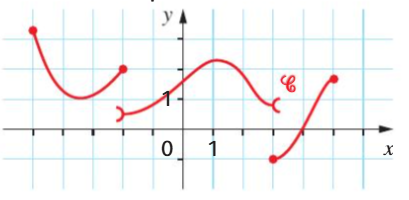
\includegraphics[scale=0.8]{Img-Exo-Obl-01}
	\end{center}
	
	Préciser si les affirmations suivantes sont vraies ou fausses.
	\begin{enumMet}
		\item La fonction $f$ est discontinue en 3 .
		
		\begin{corrBox}
			\textbf{Vrai.} La courbe présente un \og saut \fg{} en $x=3$ : on ne peut pas la tracer sans lever le crayon en ce point. La fonction $f$ est donc discontinue en $3$.
		\end{corrBox}
		
		\item La fonction $f$ est continue en 1 .
		
		\begin{corrBox}
			\textbf{Vrai.} Au voisinage de $x=1$, la courbe se trace sans lever le crayon. La fonction $f$ est continue en $1$.
		\end{corrBox}
		
		\item La fonction $f$ est continue sur l'intervalle $[-3 ; 3]$.
		
		\begin{corrBox}
			\textbf{Faux.} La courbe présente un saut en $x=-2$ (et en $x=3$). Or $-2\in[-3;3]$, donc $f$ n'est pas continue sur $[-3;3]$.
		\end{corrBox}
		
		\item La fonction $f$ est continue sur l'intervalle $]-2 ; 3[$.
		
		\begin{corrBox}
			\textbf{Vrai.} Sur l'intervalle ouvert $]-2;3[$, la courbe se trace sans lever le crayon (les points d'abscisses $-2$ et $3$ sont exclus). La fonction $f$ est continue sur $]-2;3[$.
		\end{corrBox}
		
		\item La fonction $f$ est continue sur l'intervalle $[-5 ; 2]$.
		
		\begin{corrBox}
			\textbf{Faux.} La courbe présente un saut en $x=-2$ et $-2\in[-5;2]$. La fonction $f$ n'est donc pas continue sur $[-5;2]$.
		\end{corrBox}
	\end{enumMet}
	
	%=====================================================
	\exerciceDS{}
	
	On considère la fonction $f: x \mapsto \begin{cases}6 x+8 & \text { si } x \leqslant-1 \\ -3 x+7 & \text { si }-1<x<2  \\ x-1 & \text { si } x \geqslant 2\end{cases}$
	
	La fonction $f$ est-elle continue en $-1$? et en $2$?
	
	\begin{corrBox}
		\textbf{Continuité en $\bm{-1}$ :}
		
		D'une part, $f(-1)=6 \times(-1)+8=2$.
		
		D'autre part, $\displaystyle\lim _{x \to (-1)^{+}} f(x)=\lim _{x \to (-1)^{+}} (-3x+7)=-3 \times(-1)+7=10$.
		
		Comme $\displaystyle\lim _{x \to (-1)^{+}} f(x)\neq f(-1)$, la fonction $f$ \textbf{n'est pas continue en $\bm{-1}$}.
	\end{corrBox}
	
	\begin{corrBox}
		\textbf{Continuité en $\bm{2}$ :}
		
		D'une part, $f(2)=2-1=1$.
		
		D'autre part, $\displaystyle\lim _{x \to 2^{-}} f(x)=\lim _{x \to 2^{-}} (-3x+7)=-3 \times 2+7=1$.
		
		Enfin, $\displaystyle\lim _{x \to 2^{+}} f(x)=\lim _{x \to 2^{+}} (x-1)=2-1=1$.
		
		Comme $\displaystyle\lim _{x \to 2^{-}} f(x)=\lim _{x \to 2^{+}} f(x)=f(2)$, la fonction $f$ \textbf{est continue en $\bm{2}$}.
	\end{corrBox}
	
	%=====================================================
	\exerciceDS{}
	
	On considère la fonction $f: x \mapsto\left\{\begin{array}{ll}\dfrac{1}{2} x-3 & \text { si } x \leqslant-2 \\ x+1 & \text { sinon }\end{array}\right.$ définie sur $\mathbb{R}$.
	\begin{enumMet}
		\item Montrer que la fonction $f$ n'est pas continue en -2 .
		
		\begin{corrBox}
			D'une part, $f(-2)=\dfrac{1}{2} \times(-2)-3=-1-3=-4$.
			
			D'autre part, $\displaystyle\lim _{x \to (-2)^{+}} f(x)=\lim _{x \to (-2)^{+}} (x+1)=-2+1=-1$.
			
			Comme $\displaystyle\lim _{x \to (-2)^{+}} f(x)\neq f(-2)$, la fonction $f$ n'est pas continue en $-2$.
		\end{corrBox}
		
		\item Tracer la courbe représentative de la fonction $f$ dans un repère orthonormé.
		
		\begin{corrBox}
			Sur $]-\infty;-2]$, la courbe est une portion de la droite d'équation $y=\dfrac{1}{2}x-3$ (passant par $(-6;-6)$ et $(-2;-4)$, point inclus).
			
			Sur $]-2;+\infty[$, la courbe est une portion de la droite d'équation $y=x+1$ (passant par $(0;1)$ et $(-2;-1)$, point exclu).
			
			\begin{center}
				\begin{tikzpicture}[scale=0.5]
					\draw[gray!30] (-8,-8) grid (5,6);
					\draw[->,thick] (-8,0) -- (5,0) node[below left] {$x$};
					\draw[->,thick] (0,-8) -- (0,6) node[below left] {$y$};
					\foreach \x in {-8,-6,-4,-2,2,4} \draw (\x,0.1) -- (\x,-0.1) node[below] {\footnotesize $\x$};
					\foreach \y in {-8,-6,-4,-2,2,4} \draw (0.1,\y) -- (-0.1,\y) node[left] {\footnotesize $\y$};
					\node[below left] at (0,0) {\footnotesize $0$};
					% partie gauche
					\draw[very thick, red] (-8,-7) -- (-2,-4);
					% partie droite
					\draw[very thick, red] (-2,-1) -- (5,6);
					% points
					\fill[red] (-2,-4) circle (5pt);
					\draw[red, thick, fill=white] (-2,-1) circle (5pt);
					\node[red] at (3,2.5) {$C_f$};
				\end{tikzpicture}
			\end{center}
		\end{corrBox}
	\end{enumMet}
	
	%=====================================================
	\exerciceDS{}
	
	Soit $a$ et $b$ deux réels. On considère la fonction $f: x \mapsto\left\{\begin{array}{ll}a x^2+b x+1 & \text { si } x<1 \\ x^2+a x+b & \text { si } x \geqslant 1\end{array}\right.$.
	
	Montrer que la fonction $f$ est continue sur $\mathbb{R}$.
	
	\begin{corrBox}
		Sur $]-\infty ; 1[$ et sur $] 1 ;+\infty[$, $f$ est une fonction polynôme, donc continue. Il reste à étudier la continuité en $1$.
		
		D'une part, $f(1)=1^2+a \times 1+b=1+a+b$.
		
		D'autre part, $\displaystyle\lim _{x \to 1^{-}} f(x)=a \times 1^2+b \times 1+1=a+b+1$.
		
		Enfin, $\displaystyle\lim _{x \to 1^{+}} f(x)=1^2+a\times 1+b=1+a+b$.
		
		Ainsi $\displaystyle\lim _{x \to 1^{-}} f(x)=\lim _{x \to 1^{+}} f(x)=f(1)$ : $f$ est continue en $1$.
		
		Finalement, quelles que soient les valeurs de $a$ et $b$, $f$ est continue sur $\mathbb{R}$.
	\end{corrBox}
	
	%=====================================================
	\exerciceDS{}
	
	Pour tout réel $x$, on pose $f(x)=x^5-2 x-4$.
	\begin{enumMet}
		\item Calculer $f(1)$ et $f(2)$
		
		\begin{corrBox}
			$f(1)=1^5-2\times 1-4=1-2-4=-5$
			
			$f(2)=2^5-2\times 2-4=32-4-4=24$
		\end{corrBox}
		
		\item En déduire que l'équation $x^5=2 x+4$ possède au moins une solution sur $[1 ; 2]$.
		
		\begin{corrBox}
			$x^5=2x+4 \iff x^5-2x-4=0 \iff f(x)=0$.
			
			La fonction $f$ est une fonction polynôme, donc elle est continue sur $[1;2]$.
			
			De plus, $f(1)=-5<0$ et $f(2)=24>0$, donc $0$ est compris entre $f(1)$ et $f(2)$.
			
			D'après le théorème des valeurs intermédiaires, il existe au moins un réel $c \in[1 ; 2]$ tel que $f(c)=0$, c'est-à-dire $c^5=2c+4$.
			
			L'équation $x^5=2x+4$ possède donc au moins une solution sur $[1;2]$.
		\end{corrBox}
		
		\item Donner une solution de cette équation au centième près.
		
		\begin{corrBox}
			À l'aide de la calculatrice (tableau de valeurs ou balayage) :
			
			$f(1{,}47)\approx-0{,}08<0$ \quad et \quad $f(1{,}48)\approx 0{,}14>0$.
			
			Donc $1{,}47<c<1{,}48$, soit $\mRouge{c\approx 1{,}47}$ au centième près.
		\end{corrBox}
	\end{enumMet}
	
	%=====================================================
	\exerciceDS{}
	
	On considère la fonction $f: x \mapsto e^x-3 x$, définie sur $\mathbb{R}$.
	\begin{enumMet}
		\item Justifier que $f$ est continue et dérivable sur $\mathbb{R}$ et déterminer $f^{\prime}(x)$ pour tout réel $x$
		
		\begin{corrBox}
			La fonction $f$ est dérivable sur $\mathbb{R}$ comme somme de fonctions dérivables sur $\mathbb{R}$ ($x\mapsto e^x$ et $x\mapsto -3x$). Étant dérivable sur $\mathbb{R}$, elle est continue sur $\mathbb{R}$.
			
			Pour tout réel $x$ : $f^{\prime}(x)=e^x-3$.
		\end{corrBox}
		
		\item Quel est le sens de variation de $f$ sur l'intervalle $[0 ; 1]$ ?
		
		\begin{corrBox}
			Si $0 \leqslant x \leqslant 1$, alors, par croissance de la fonction exponentielle sur $\mathbb{R}$, $e^0 \leqslant e^x \leqslant e^1$, soit $1\leqslant e^x\leqslant e$.
			
			Donc $e^x-3 \leqslant e-3<0$ (car $e\approx 2{,}718$).
			
			Ainsi $f'(x)<0$ sur $[0;1]$ : la fonction $f$ est \textbf{strictement décroissante sur $\bm{[0 ; 1]}$}.
		\end{corrBox}
		
		\item Que vaut $f(0)$ ? Quel est le signe de $f(1)$ ?
		
		\begin{corrBox}
			$f(0)=e^0-3\times 0=1$
			
			$f(1)=e-3\approx-0{,}28$, donc $f(1)<0$.
		\end{corrBox}
		
		\item En déduire que l'équation $e^x=3 x$ admet exactement une solution sur $[0 ; 1]$.
		
		\begin{corrBox}
			$e^x=3x \iff e^x-3x=0\iff f(x)=0$.
			
			Sur $[0;1]$ :
			\begin{itemMet}
				\item $f$ est continue ;
				\item $f$ est strictement décroissante ;
				\item $f(0)=1>0$ et $f(1)<0$, donc $0$ est compris entre $f(1)$ et $f(0)$.
			\end{itemMet}
			D'après le corollaire du théorème des valeurs intermédiaires (pour les fonctions strictement monotones), l'équation $f(x)=0$, c'est-à-dire $e^x=3x$, admet \textbf{exactement une solution} sur $[0;1]$.
		\end{corrBox}
	\end{enumMet}
	
	%=====================================================
	\exerciceDS{}
	
	On considère la fonction $f: x \mapsto 2 x^3+9 x^2-60 x+3$, définie sur $\mathbb{R}$.
	\begin{enumMet}
		\item Étudier les variations de la fonction $f$.
		
		\begin{corrBox}
			La fonction $f$ est dérivable sur $\mathbb{R}$ (fonction polynôme). Pour tout réel $x$ :
			\[f^{\prime}(x)=6 x^2+18 x-60=6\left(x^2+3 x-10\right)\]
			Pour le trinôme $x^2+3x-10$ : $\Delta=3^2-4\times1\times(-10)=49>0$, d'où deux racines :
			\[x_1=\dfrac{-3-7}{2}=-5 \qquad x_2=\dfrac{-3+7}{2}=2\]
			Le trinôme est du signe de $a=1>0$ à l'extérieur des racines.
			
			$f(-5)=2\times(-125)+9\times25-60\times(-5)+3=-250+225+300+3=278$
			
			$f(2)=2\times8+9\times4-60\times2+3=16+36-120+3=-65$
			
			De plus, $\displaystyle\lim _{x \to -\infty} f(x)=-\infty$ et $\displaystyle\lim _{x \to +\infty} f(x)=+\infty$ (limites du terme de plus haut degré $2x^3$).
			
			\begin{center}
				\begin{tikzpicture}
					\tkzTabInit[lgt=2,espcl=3]{$x$/1,$f'(x)$/1,$f$/2}{$-\infty$,$-5$,$2$,$+\infty$}
					\tkzTabLine{,+,z,-,z,+,}
					\tkzTabVar{-/$-\infty$,+/$278$,-/$-65$,+/$+\infty$}
				\end{tikzpicture}
			\end{center}
		\end{corrBox}
		
		\item En déduire la nombre de solutions de l'équation $f(x)=0$ sur $\mathbb{R}$.
		
		\begin{corrBox}
			\textbf{Sur $\bm{]-\infty ;-5]}$ :} $f$ est continue et strictement croissante, $\displaystyle\lim _{x \to -\infty} f(x)=-\infty$ et $f(-5)=278>0$. D'après le corollaire du théorème des valeurs intermédiaires, l'équation $f(x)=0$ admet une unique solution sur cet intervalle.
			
			\textbf{Sur $\bm{[-5 ; 2]}$ :} $f$ est continue et strictement décroissante, $f(-5)=278>0$ et $f(2)=-65<0$. L'équation $f(x)=0$ admet une unique solution sur cet intervalle.
			
			\textbf{Sur $\bm{[2 ;+\infty[}$ :} $f$ est continue et strictement croissante, $f(2)=-65<0$ et $\displaystyle\lim _{x \to +\infty} f(x)=+\infty$. L'équation $f(x)=0$ admet une unique solution sur cet intervalle.
			
			Ainsi, l'équation $f(x)=0$ possède \textbf{exactement 3 solutions} sur $\mathbb{R}$.
		\end{corrBox}
	\end{enumMet}
	
	%=====================================================
	\exerciceDS{}
	
	Soit $g$ la fonction définie sur $[-3 ; 6]$ par :
	$$
	g(x)=\frac{1}{3} x^3-x-8
	$$
	
	\begin{enumMet}
		\item Dresser le tableau de variations de la fonction $g$.
		
		\begin{corrBox}
			$g$ est dérivable sur $[-3;6]$ (fonction polynôme) et pour tout $x\in[-3;6]$ :
			\[g'(x)=\dfrac{1}{3}\times 3x^2-1=x^2-1=(x-1)(x+1)\]
			$g'(x)=0 \iff x=-1$ ou $x=1$. Le trinôme est positif à l'extérieur des racines et négatif entre elles.
			
			$g(-3)=\dfrac{1}{3}\times(-27)+3-8=-9+3-8=-14$
			
			$g(-1)=-\dfrac{1}{3}+1-8=-\dfrac{22}{3}\approx-7{,}33$
			
			$g(1)=\dfrac{1}{3}-1-8=-\dfrac{26}{3}\approx-8{,}67$
			
			$g(6)=\dfrac{1}{3}\times216-6-8=72-14=58$
			
			\begin{center}
				\begin{tikzpicture}
					\tkzTabInit[lgt=2,espcl=3]{$x$/1,$g'(x)$/1,$g$/2}{$-3$,$-1$,$1$,$6$}
					\tkzTabLine{,+,z,-,z,+,}
					\tkzTabVar{-/$-14$,+/$-\frac{22}{3}$,-/$-\frac{26}{3}$,+/$58$}
				\end{tikzpicture}
			\end{center}
		\end{corrBox}
		
		\item Montrer que l'équation $g(x)=0$ admet une solution unique $\alpha$ dans $[-3 ; 6]$. Déterminer un encadrement de $\alpha$ au millième près.
		
		\begin{corrBox}
			\textbf{Sur $\bm{[-3;1]}$ :} d'après le tableau de variations, le maximum de $g$ est $-\dfrac{22}{3}<0$. Donc $g(x)<0$ et l'équation $g(x)=0$ n'a pas de solution sur cet intervalle.
			
			\textbf{Sur $\bm{[1;6]}$ :} $g$ est continue et strictement croissante, $g(1)=-\dfrac{26}{3}<0$ et $g(6)=58>0$. D'après le corollaire du théorème des valeurs intermédiaires, l'équation $g(x)=0$ admet une unique solution $\alpha$ sur $[1;6]$.
			
			Conclusion : l'équation $g(x)=0$ admet une unique solution $\alpha$ dans $[-3;6]$.
			
			\medskip
			À la calculatrice : $g(3{,}229)\approx-0{,}007<0$ et $g(3{,}230)\approx0{,}003>0$.
			
			Donc $\mRouge{3{,}229<\alpha<3{,}230}$.
		\end{corrBox}
		
		\item En déduire le tableau de signes de $g$ sur $[-3 ; 6]$.
		
		\begin{corrBox}
			$g(x)<0$ sur $[-3;1]$ ; sur $[1;6]$, $g$ est strictement croissante et s'annule en $\alpha$, donc $g(x)<0$ sur $[1;\alpha[$ et $g(x)>0$ sur $]\alpha;6]$.
			
			\begin{center}
				\begin{tikzpicture}
					\tkzTabInit[lgt=2,espcl=3]{$x$/1,$g(x)$/1}{$-3$,$\alpha$,$6$}
					\tkzTabLine{,-,z,+,}
				\end{tikzpicture}
			\end{center}
		\end{corrBox}
	\end{enumMet}
	
	%=====================================================
	\exerciceDS{}
	
	Soit $f$ la fonction définie sur $[-2 ; 1]$ par:
	$$
	f(x)=\mathrm{e}^{3 x}-3 x+1
	$$
	
	\begin{enumMet}
		\item Dresser le tableau de variations de la fonction $f$.
		
		\begin{corrBox}
			$f$ est dérivable sur $[-2;1]$ et pour tout $x\in[-2;1]$ :
			\[f'(x)=3\mathrm{e}^{3x}-3=3\left(\mathrm{e}^{3x}-1\right)\]
			$\mathrm{e}^{3x}-1>0 \iff \mathrm{e}^{3x}>1 \iff \mathrm{e}^{3x}>\mathrm{e}^0 \iff 3x>0 \iff x>0$.
			
			Donc $f'(x)<0$ sur $[-2;0[$, $f'(0)=0$ et $f'(x)>0$ sur $]0;1]$.
			
			$f(-2)=\mathrm{e}^{-6}+6+1=\mathrm{e}^{-6}+7\approx7{,}002$
			
			$f(0)=\mathrm{e}^0-0+1=2$
			
			$f(1)=\mathrm{e}^3-3+1=\mathrm{e}^3-2\approx18{,}09$
			
			\begin{center}
				\begin{tikzpicture}
					\tkzTabInit[lgt=2,espcl=3.5]{$x$/1,$f'(x)$/1,$f$/2}{$-2$,$0$,$1$}
					\tkzTabLine{,-,z,+,}
					\tkzTabVar{+/$\mathrm{e}^{-6}+7$,-/$2$,+/$\mathrm{e}^{3}-2$}
				\end{tikzpicture}
			\end{center}
		\end{corrBox}
		
		\item Déterminer le nombre de solutions de l'équation $f(x)=3$ sur l'intervalle $[-2 ; 1]$.
		
		\begin{corrBox}
			\textbf{Sur $\bm{[-2;0]}$ :} $f$ est continue et strictement décroissante, $f(-2)\approx7{,}002>3$ et $f(0)=2<3$. D'après le corollaire du théorème des valeurs intermédiaires, l'équation $f(x)=3$ admet une unique solution $x_1$ sur cet intervalle.
			
			\textbf{Sur $\bm{[0;1]}$ :} $f$ est continue et strictement croissante, $f(0)=2<3$ et $f(1)\approx18{,}09>3$. L'équation $f(x)=3$ admet une unique solution $x_2$ sur cet intervalle.
			
			L'équation $f(x)=3$ admet donc \textbf{exactement deux solutions} sur $[-2;1]$.
		\end{corrBox}
		
		\item Donner une valeur approchée au centième de chacune des solutions de l'équation $f(x)=3$.
		
		\begin{corrBox}
			À l'aide de la calculatrice :
			
			$f(-0{,}62)\approx3{,}016>3$ et $f(-0{,}61)\approx2{,}990<3$, donc $-0{,}62<x_1<-0{,}61$ et $\mRouge{x_1\approx-0{,}61}$.
			
			$f(0{,}38)\approx2{,}987<3$ et $f(0{,}39)\approx3{,}052>3$, donc $0{,}38<x_2<0{,}39$ et $\mRouge{x_2\approx0{,}38}$.
		\end{corrBox}
	\end{enumMet}
	
	%=====================================================
	\exerciceDS{}
	
	On injecte du glucose à un patient.
	On estime que la glycémie, en gramme par litre de sang, au bout de $t$ heures est modélisée par la fonction $f$ définie sur [ $0 ; 7$ ] par :
	$$
	f(t)=0,6 \mathrm{e}^{-0,8 t}+0,84
	$$
	
	\begin{enumMet}
		\item Déterminer la glycémie au moment de l'injection.
		
		\begin{corrBox}
			Au moment de l'injection, $t=0$ :
			\[f(0)=0{,}6\,\mathrm{e}^{0}+0{,}84=0{,}6+0{,}84=1{,}44\]
			La glycémie au moment de l'injection est de $\mRouge{1{,}44}$ g/L.
		\end{corrBox}
		
		\item Étudier le sens de variation de $f$. Interpréter.
		
		\begin{corrBox}
			$f$ est dérivable sur $[0;7]$ et pour tout $t\in[0;7]$ :
			\[f'(t)=0{,}6\times(-0{,}8)\,\mathrm{e}^{-0{,}8t}=-0{,}48\,\mathrm{e}^{-0{,}8t}\]
			Comme $\mathrm{e}^{-0{,}8t}>0$ pour tout réel $t$, on a $f'(t)<0$ sur $[0;7]$.
			
			La fonction $f$ est donc strictement décroissante sur $[0;7]$.
			
			\textbf{Interprétation :} après l'injection, la glycémie du patient diminue au cours du temps (de $1{,}44$ g/L à environ $f(7)\approx0{,}84$ g/L).
		\end{corrBox}
		
		\item À l'aide de la calculatrice, déterminer, à $0,1 \mathrm{~h}$ près, le temps au bout duquel :
		\begin{enumMet}
			\item la glycémie descend à 1,24 gramme par litre ;
			
			\begin{corrBox}
				On cherche $t$ tel que $f(t)=1{,}24$.
				
				$f$ est continue et strictement décroissante sur $[0;7]$, avec $f(0)=1{,}44>1{,}24$ et $f(7)\approx0{,}842<1{,}24$ : d'après le corollaire du théorème des valeurs intermédiaires, cette équation admet une unique solution sur $[0;7]$.
				
				À la calculatrice : $f(0{,}5)\approx1{,}242>1{,}24$ et $f(0{,}6)\approx1{,}211<1{,}24$.
				
				La glycémie descend à $1{,}24$ g/L au bout d'environ $\mRouge{0{,}5}$ \textbf{heure}.
			\end{corrBox}
			
			\item la glycémie aura diminué de 0,5 gramme par litre.
			
			\begin{corrBox}
				La glycémie aura diminué de $0{,}5$ g/L lorsqu'elle vaudra $1{,}44-0{,}5=0{,}94$ g/L. On cherche donc $t$ tel que $f(t)=0{,}94$.
				
				Comme précédemment, $f(0)=1{,}44>0{,}94$ et $f(7)\approx 0{,}842<0{,}94$ : l'équation admet une unique solution sur $[0;7]$.
				
				À la calculatrice : $f(2{,}2)\approx0{,}943>0{,}94$ et $f(2{,}3)\approx0{,}935<0{,}94$.
				
				La glycémie aura diminué de $0{,}5$ g/L au bout d'environ $\mRouge{2{,}2}$ \textbf{heures}.
			\end{corrBox}
		\end{enumMet}
	\end{enumMet}
	
	%=====================================================
	\exerciceDS{}
	
	À la suite d'un accident industriel, un gaz se répand dans un local d'usine. On admet qu'au-delà de six minutes il n'y a quasiment plus de gaz dans l'air.
	On modélise l'évolution du taux de gaz dans l'air grâce à la fonction $f$ définie sur $[0 ; 6]$ par :
	$$
	f(x)=2 x \mathrm{e}^{-x}
	$$
	où $x$ est le nombre de minutes écoulées depuis l'accident et $f(x)$ le taux de gaz dans l'air exprimé en partie par million (ppm).
	On donne la courbe représentative $C$ de la fonction $f$ sur $[0 ; 6]$.
	
	\begin{center}
		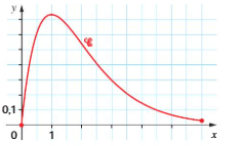
\includegraphics[scale=1.2]{Img-Exo-Obl-03}
	\end{center}
	
	\begin{enumMet}
		\item Déterminer le tableau complet des variations de la fonction $f$ sur l'intervalle $[0 ; 6]$.
		
		\begin{corrBox}
			$f$ est dérivable sur $[0;6]$. On pose $u(x)=2x$ et $v(x)=\mathrm{e}^{-x}$, d'où $u'(x)=2$ et $v'(x)=-\mathrm{e}^{-x}$.
			\[f'(x)=2\mathrm{e}^{-x}+2x\times\left(-\mathrm{e}^{-x}\right)=2\mathrm{e}^{-x}-2x\mathrm{e}^{-x}=2(1-x)\mathrm{e}^{-x}\]
			Comme $2\mathrm{e}^{-x}>0$, $f'(x)$ est du signe de $1-x$ : positif sur $[0;1[$, nul en $1$, négatif sur $]1;6]$.
			
			$f(0)=0$ \qquad $f(1)=2\mathrm{e}^{-1}=\dfrac{2}{\mathrm{e}}\approx0{,}736$ \qquad $f(6)=12\mathrm{e}^{-6}\approx0{,}030$
			
			\begin{center}
				\begin{tikzpicture}
					\tkzTabInit[lgt=2,espcl=3.5]{$x$/1,$1-x$/1,$f'(x)$/1,$f$/2}{$0$,$1$,$6$}
					\tkzTabLine{,+,z,-,}
					\tkzTabLine{,+,z,-,}
					\tkzTabVar{-/$0$,+/$\frac{2}{\mathrm{e}}$,-/$12\mathrm{e}^{-6}$}
				\end{tikzpicture}
			\end{center}
		\end{corrBox}
		
		\item \begin{enumMet}
			\item Montrer que l'équation $f(x)=0,65$ admet deux solutions $x_1$ et $x_2$ sur [ $0 ; 6$ ], avec $x_1<x_2$.
			
			\begin{corrBox}
				\textbf{Sur $\bm{[0;1]}$ :} $f$ est continue et strictement croissante, $f(0)=0<0{,}65$ et $f(1)\approx0{,}736>0{,}65$. D'après le corollaire du théorème des valeurs intermédiaires, l'équation $f(x)=0{,}65$ admet une unique solution $x_1$ sur $[0;1]$.
				
				\textbf{Sur $\bm{[1;6]}$ :} $f$ est continue et strictement décroissante, $f(1)\approx0{,}736>0{,}65$ et $f(6)\approx0{,}030<0{,}65$. L'équation $f(x)=0{,}65$ admet une unique solution $x_2$ sur $[1;6]$.
				
				L'équation $f(x)=0{,}65$ admet donc exactement deux solutions $x_1$ et $x_2$ sur $[0;6]$, avec $x_1<1<x_2$.
			\end{corrBox}
			
			\item À l'aide de la calculatrice, donner une valeur approchée de $x_1$ et de $x_2$ à 0,1 minute près.
			
			\begin{corrBox}
				$f(0{,}5)\approx0{,}607<0{,}65$ et $f(0{,}6)\approx0{,}659>0{,}65$, donc $0{,}5<x_1<0{,}6$ et $\mRouge{x_1\approx0{,}6}$ min.
				
				$f(1{,}5)\approx0{,}669>0{,}65$ et $f(1{,}6)\approx0{,}646<0{,}65$, donc $1{,}5<x_2<1{,}6$ et $\mRouge{x_2\approx1{,}6}$ min.
			\end{corrBox}
		\end{enumMet}
		
		\item On considère que le gaz a un effet irritant pour l'organisme si le taux dépasse $0,65 \mathrm{ppm}$ pendant plus d'une minute.
		
		Déterminer si le personnel de l'usine a été affecté ou non par la fuite de gaz, en explicitant la démarche.
		
		\begin{corrBox}
			D'après le tableau de variations, $f(x)>0{,}65$ si et seulement si $x\in\,]x_1;x_2[$. Le taux dépasse donc $0{,}65$ ppm pendant une durée égale à $x_2-x_1$.
			
			Avec les valeurs au dixième, on obtient $x_2-x_1\approx1{,}6-0{,}6=1$ : cette précision \textbf{ne permet pas de conclure}. Il faut affiner les encadrements à la calculatrice :
			
			$f(0{,}581)\approx0{,}64995<0{,}65$ et $f(0{,}582)\approx0{,}65042>0{,}65$, donc $0{,}581<x_1<0{,}582$.
			
			$f(1{,}583)\approx0{,}65016>0{,}65$ et $f(1{,}584)\approx0{,}64992<0{,}65$, donc $1{,}583<x_2<1{,}584$.
			
			On en déduit :
			\[x_2-x_1>1{,}583-0{,}582=1{,}001>1\]
			Le taux de gaz a dépassé $0{,}65$ ppm pendant un peu plus d'une minute : \textbf{le personnel de l'usine a donc été affecté} par la fuite de gaz (de justesse).
		\end{corrBox}
	\end{enumMet}
	
\end{document}